\documentclass[a4paper,11pt,notitlepage]{report}
%fleqn

\usepackage[italian]{babel}
\usepackage{amsmath, amssymb}
\usepackage{amsthm}
\usepackage{amstext}
\usepackage{array}
\usepackage{graphicx,color,psfrag,pgfplots}
\usepackage[tight]{subfigure}
\usepackage[bf,small]{caption}
\usepackage{bbm}
\usepackage{wrapfig}
%\usepackage[top=2in, bottom=1.5in, left=1in, right=1in]{geometry}

\usepackage{natbib}

%%%%%%%%%%%%%%PER IL BOX
\usepackage{tikz}
\usetikzlibrary{shapes,positioning,arrows,calc,shadows}
\tikzstyle{abstractbox} = [draw=black, fill=white, rectangle, 
  inner sep=11pt, style=rounded corners]%, drop shadow={fill=black,
  %opacity=1}]
  \tikzstyle{abstracttitle}=[fill=white]
  \newcommand{\mybox}[3][fill=white]{
    \begin{center}
      \begin{tikzpicture}
        \node [abstractbox, #1] (box)
        {\begin{minipage}{0.95\linewidth}
%           \setlength{\parindent}{2mm}
           \footnotesize #2
          \end{minipage}};
        \node[abstracttitle, right=11pt] at (box.north west) {#3};
      \end{tikzpicture}
    \end{center}
  }
%%%%%%%%FINE PER IL BOX


%%%%%%%%%%%%%%%%%%%%%%%%%%%%%%%%%%
\usepackage{listings}
\usepackage{color}

\definecolor{mygreen}{rgb}{0,0.6,0}
\definecolor{mygray}{rgb}{0.5,0.5,0.5}
\definecolor{mymauve}{rgb}{0.58,0,0.82}


\lstdefinestyle{customc}{
  belowcaptionskip=1\baselineskip,
  breaklines=true,
  frame=single,
  xleftmargin=\parindent,
  language=C++,
  showstringspaces=false,
  basicstyle=\footnotesize\ttfamily,
  keywordstyle=\bfseries\color{green!40!black},
  commentstyle=\itshape\color{purple!40!black},
  identifierstyle=\color{black},
  stringstyle=\color{purple},
  %morekeywords={}  
}

\lstdefinestyle{customasm}{
  belowcaptionskip=1\baselineskip,
  frame=L,
  xleftmargin=\parindent,
  language=[x86masm]Assembler,
  basicstyle=\footnotesize\ttfamily,
  commentstyle=\itshape\color{purple!40!black},
}


\lstdefinestyle{general}{ %
  backgroundcolor=\color{white},
  basicstyle=\footnotesize,       
  breakatwhitespace=false,       
  breaklines=true,                 
  %captionpos=t,
  abovecaptionskip=-0.8cm,
  %belowcaptionskip=-0.8cm,
  commentstyle=\color{mygreen},
  deletekeywords={...},            
  escapeinside={\%*}{*)},
  extendedchars=true,   
  frame=lines,
  %none L false leftline  topline bottomline shadowbox single lines 
  keepspaces=true,                
  keywordstyle=\color{blue},       
  language=C++,                 
  morekeywords={Real,UInt},           
  %numbers=left,
  %numbersep=5pt,              
  %numberstyle=\tiny\color{mygray}, 
  rulecolor=\color{black},
  showspaces=false,        
  showstringspaces=false,         
  showtabs=false,                  
  %stepnumber=1,                   
  stringstyle=\color{mymauve},
  tabsize=2,                      
  title=\lstname                  
}

\lstset{escapechar=@,style=customc}
%%%%%%%%%%%%%%%%%%%%%%%%%%
\usepackage{booktabs}
\usepackage{enumitem}
\usetikzlibrary{patterns}
\theoremstyle{plain}
\newtheorem{teorema}{Teorema}
\graphicspath{{img/}}
\usepackage{textcomp}
\usetikzlibrary{calc,decorations.markings,positioning}
\usepackage{mathtools}
%Per togliere i numeri alle equazioni
%\mathtoolsset{showonlyrefs}

\newcommand{\vect}[1]{\mathbf{#1}}
\newcommand{\classe}[1]{\emph{#1}}
\newcommand{\referenza}[1]{[\ref{#1}]}
\newcommand{\referenzaeq}[1]{(\ref{#1})}
\newcommand{\figref}[1]{( Fig.\ref{#1} )}
\newcommand{\nsp}[1]{\foreach \n in {1,...,#1}{\!}}
\newcommand{\psp}[1]{\foreach \n in {1,...,#1}{\,}}	

\begin{document}

%\begin{titlepage}
\begin{center}
    { \scshape 
    Laurea magistrale\\
    in ingegneria matematica\\
    }
\end{center}
\vspace{1.2cm}
\begin{flushleft}
		\Large
		Elaborato di Tesi ...
		\vspace{1.5cm}
\end{flushleft}
\begin{figure}[h]
		\centering
		
\includegraphics[width=0.25\textwidth]{Varie/logo-polimi}
		\vspace{1cm}
\end{figure}
\begin{center}
{ \bfseries  {\Large Titolo progetto di tesi ...}\\
\vspace{0.2cm} }
\end{center}
\vspace{0.4cm}
\begin{flushright}
		\Large
		Progetto svolto da:\\
		Andrea Bortolossi\\
		Matr. 783023\\
		\vspace{1.5cm}
\end{flushright}
\begin{center}
Anno Accademico 2013--2014
\end{center}

\end{titlepage}
%\clearpage
%\tableofcontents
%\chapter{Introduction}
\section{Brief history of VLSI devices}


In 1947 John Bardeen, William Shockley and Walter Brattain (three scientists of Bell Telephone Labs) invented the bipolar transistor and since that crucial point there has been a growth  of the semiconductor industry never known before, with serious impact on the way people work and live today. 

Before reach the functionality and the miniaturization of modern devices, some fundamental steps has been made.
In 1958 was produced the first intagrated circuits (IC)  followed by the introduction of the first MOSFET(1960) and CMOS(1963). Into these inventions the first micro-processor(1971) sank his roots  and since that time until present, an ever-increasing progress has continued, according to the indication of \textit{Moore's Law} (formulated by Gordton Moore in 1965).

These events led microelectronic industry at the doors of the VLSI era (Very-Large-Scale-Integration). Indeed in the last thirty years the benefits of miniaturization have been the key in the evolutionary progress leading to today's computers, wireless units, and comunication systems that offer superior performance, dramatically reduced cost per function, and much reduced physical size.

The large worldwide investment in VLSI technology constitutes a formidable driving force that guarantee the continued progress in IC integration density and speed, for as long as physical principles will allow.

\section{Why FEMOS}

From this point we want start and remark that the aim of numerical simulations is the full comprehension of the physical phenomenon which lies behind the function of modern device. As already underlying this situation became rapidly more important since in the last years devices became more complex and in many cases compact models are insufficent to fully describe the behavoiur of devices.

Even if there's exist many commercial software which are able to resolve different physic situations, it's really difficult satisfy the necessities of industries. A simulator should be more desireable if it  could couple any kind of equations but this is a far ahievement. Modern software are often specialized on precise physic branch. Obviously this strategic choice guarantees more efficiency but it implies a lost in generality. The conseguence is that the work of the model analyst became harder when he have to afford problems located in the middle of different phenomenon. 

Consider for a moment to analyse the funcionality of a new device, which its electric behaviour is strong influeced by its mechanic response. Basically you are interested to the resolution of Maxwell's law  (which is well performed by SDEVICE simulator) and the Navier-Lam\`e equations (which is well performed by COMSOL simulator). Now the question is: how to put in comunication the different outputs?
Take into account that it's not possbile known precisely how the above programs resolves the equations, which implies a relevant risk when you decide to combine the solutions. 
In other words the development of an own code is at least desirable and possibly helpful. The main advantage is the total control on simulation procedure and the possibility of fully customize. Although the major drawback is that the improvement of a personal code needs time and human resources, which in many cases are not avaible.   

The FEMOS project (\textit{Finite Element Method Oriented Solver}) sinks its motivations in the above framework. The main intention is to solve different physics aspects and give a more precise description of devices with a single output. The complexity of this achievement guarantees a continuum source of physic, numerical and programming challenges. 
Between them, even if modern devices present innovative and unexpected behaviour, we can't avoid the treatment of the classical semiconductor devices from the simulation possibilties of FEMOS.
This thesis found its origin in the development of this achievement, but as subject covered a spread wide area in terms of models and kind of devices, we decide to focus on precise points which we present here:
\begin{itemize}
\item development of a finite element based simulator for semiconductor devices which deals with multiple generation/recombination and mobility models;
\item check solutions obtained against commercial software (SDEVICE);
\item definition and implementation of a new way to compute the current density inside the device;
\item extension of the residual method presented in \textcolor{red}{referenza} for the 3D case;
\item evaluation of the possibility to extend the residual method at the computation of the current density inside the device.
\end{itemize}


%\clearpage
%\chapter{Semiconductor model}
%
%\textcolor{blue}{O forse prima parte...dipende da quello che riusciamo a fare...nel caso la divisione fra il primo ed il secondo capitolo sarebbe approccio formulazione agli spostamenti e duale mista}
%
%\section{DD Model}
In this work we deal with mathematical modeling and numerical simulation of different semiconductor devices. 

There are several methods to model integrated devices, this project is based on a semi-classical model, in particular we work with the classical Drift-Diffusion model (DD). Maybe this kind of model is the most used for industrial simulation, due to an excellent trade-off between machine time cost and physical accuracy. Nevertheless to describe the propagation of any electromagnetic signal in a medium, we have to start from the system of Maxwell equations, which reads as follows:

\begin{equation}
\label{eq: Maxwell system}
\left\{
\begin{array}{rcl}
\nabla \times \vect{H} & = & \vect{J} + \dfrac{\partial \vect{D}}{\partial t} \\ \\
\nabla \times \vect{E} & = & - \dfrac{\partial \vect{B}}{\partial t} \\ \\
\nabla \cdot \vect{D} & = & \rho \\ \\
\nabla \vect{B} &  = & 0
\end{array}
\right.
\end{equation}

We are able to complete the system with the following set of constitutive laws that characterize the electromagnetic properties of the medium:

\begin{equation}
\begin{array}{rcl}
\vect{D} & = & \epsilon \vect{E} \\
\vect{B} & = & \mu_m \vect{H}
\end{array}
\end{equation}

From \referenzaeq{eq: Maxwell system} we elaborate the DD model, through some interesting hypostesis which are:
\begin{itemize}
\item Lorentz-Gauge for the vector potential of $\vect{B}$.
\item Quasi static approximation.
\end{itemize}

The second one is related with the IC component sizes and characteristics and it is a reasonable hypotesis for our simulations.	
The system obtained after this suitable approximation looks as follows:
\begin{equation}
\left\{
\begin{array}{rcll}
\nabla \cdot (-\epsilon \nabla \varphi) & = & \rho &\psp{15} \textit{Poisson equation}\\ \\
\dfrac{\partial \rho}{\partial t} + \nabla \cdot \vect{J} & = & 0 &\psp{15} \textit{Continuity equation}\\
\end{array}
\right.
\end{equation} 

To close the above system we need to specify the mathematical form of the electric charge density and the electric conduction current density.

It's well known that intrinsic semiconductor does not appreciably allow current flow, for this reason it's usual introducing impurities (called dopants) in the periodic structure. Dopant impurities are divided into two types: 
\begin{itemize}
\item acceptor type, wich provide positive carriers (holes);
\item donor type, wich provide negative carriers (electron). 
\end{itemize}
It is usual point out acceptor concentration with $N_A$ while donor concentration with $N_D$. However for the electric charge density formulation we are interested only in ionized impurities, thus we obtain the sequent costitutive law:
\begin{equation}
\rho = \underbrace{q(p-n)}_{\rho_{free}} +\underbrace{q(N_D^+-N_A^-)}_{\rho_{fixed}}
\end{equation}

We emphasize the two kind of charge present in the device: $\rho_{fixed}$ related to ionized impurities and $\rho_{free}$ related to free carriers in band ($p$ and $n$ are the concentration of holes and electron respectively). Notice that we assume $N_D^+$ and $N_A^-$ time invariant.

In this work we consider only the transport of these two charge carriers in the device. Consistently with this hypotesis the conduction current density can be written as:
\begin{equation}
\vect{J} = \vect{J_n} + \vect{J_p}
\end{equation}

where $J_n$ and $J_p$ are respectively the electric conduction current density of electrons and holes.
To model charge current flow we consider two principal mechanisms:
\begin{itemize}
\item Diffusion current, according to Fick's law.
\item Drift current, according to Ohm's law.
\end{itemize}
The form of these current densities is expressed by the following relations:
\begin{equation}
\begin{array}{rclcl}
\vect{J_n} & = & \overbrace{q\mu_n n \vect{E}}^{Drift} &+& \overbrace{(- qD_n(- \nabla n))}^{Diffusion} \\ \\
\vect{J_p} & = & q\mu_p p \vect{E} &+& (-qD_p \nabla p) 
\end{array}
\end{equation}



 According with the preview hypotesis and replacing the costitutive laws, we obtain the seguent DD model forumulation:
\begin{equation}
\label{eq: full problem}
\left\{
\begin{array}{rcll}
\nabla \cdot (-\epsilon \nabla \varphi) & = & q(p-n+N_D^+-N_A^-)  &\psp{15} \textit{Poisson equation}\\ \\
-q\dfrac{\partial n}{\partial t} + \nabla \cdot ( - q\mu_n n \nabla \varphi + qD_n \nabla n )& = & qR &\psp{15} \textit{Electron Continuity equaiton}\\ \\
q\dfrac{\partial p}{\partial t} + \nabla \cdot (- q\mu_p p \nabla \varphi - qD_p \nabla p )& = & -qR &\psp{15} \textit{Hole Continuity equaiton}
\end{array}
\right.
\end{equation}

The system is an incompletely parbolic initial value/boundary problem in three scalar unkown dependent variables $\varphi(\vect{x},t)$, $n(\vect{x},t)$ and $p(\vect{x},t)$. Notice that the problem is a nonlinearly coupled system of PDE's, because of the presence of the drift terms $n\nabla \varphi$ and $p \nabla 	\varphi$. 

From Maxwell equations we are able to guarantee only that $\vect{J}$ is a solenoidal field, we can't say nothing about the properties of $\vect{J_n}$ and $\vect{J_p}$. For this reason there is a new term in the right hand side. We can interpret $R(\vect{x},t)$ as the net rate of generation and recombination.

We consider also the stationary form for our purpose.

\begin{equation}
\left\{
\begin{array}{rcl}
\nabla \cdot (-\epsilon \nabla \varphi) & = & q(p-n+N_D^+-N_A^-) \\ \\
\nabla \cdot ( - q\mu_n n \nabla \varphi + qD_n \nabla n )& = & qR \\ \\
\nabla \cdot (- q\mu_p p \nabla \varphi - qD_p \nabla p )& = & -qR
\end{array}
\right.
\end{equation}
%
%\clearpage
%
%\chapter{Resolution of the system}

\section{Iteration algorithms}

The high nonlinear nature of the problem 	makes an analytical treatment very difficult, if not even impossible. For this reason, numerical schemes must be used to compute an approximate solution of the system \referenzaeq{eq: stationary problem}. Indisputably, the most used algorithms are \textit{the fully coupled Newton's method} and \textit{the decoupled Gummel map}. We spent only few words on the former as we implemented the latter, but first of all let us introduce a suitable linearization of the stationary DD equations. We can consider \referenzaeq{eq: stationary problem} in a more compact form:

\begin{equation}
\label{eq: abstract problem fully}
\vect{F(U)}=\vect{0}
\end{equation}

where:

\begin{equation}
\vect{U}:=[\varphi,n,p]^T \psp{30} \vect{F(U)}:=\left[ \begin{array}{c}
F_1(\vect{U}) \\
F_2(\vect{U}) \\
F_3(\vect{U})
\end{array}
\right]
\end{equation}

and having set:

\begin{align*}
F_1(\vect{U}) & = \nabla \cdot (-\epsilon \nabla \varphi) - q(p-n+N_D^+-N_A^-) \\
F_2(\vect{U}) & = \nabla \cdot ( - q\mu_n n \nabla \varphi + qD_n \nabla n )-qR \\
F_3(\vect{U}) & = \nabla \cdot (- q\mu_p p \nabla \varphi - qD_p \nabla p )+qR
\end{align*}

\vspace{0.1cm}

Basically the fully coupled Newton's method is an extension to differential operators of the well known Newton's method for the search of a zero for real functions ($f:\mathbb{R}\rightarrow \mathbb{R}$). In fact the vector function $\vect{F}$ is a nonlinear differential operator and the associated problem which we intend to resolve is: given a functional space $V$ and the operator $\vect{F}:V\rightarrow V$, find $\vect{U}\in V$ such that \referenzaeq{eq: abstract problem fully} is satisfied.
Just for the moment we don't care about the identity of $V$, which we will treat in details in the next section; now we are able to define  the abstract Newton's Method for the iterative solution of problem \referenzaeq{eq: stationary problem}:

\mybox{
\vspace{0.1cm}
Given $\vect{U}^0\in V$, for all $k\geq 0$ until convergence, solve the following linearized problem: 

\begin{equation}
\label{eq: abstract newton's method}
\begin{array}{c}
\vect{F'}(\vect{U}^k)\delta\vect{U}^k=-\vect{F}(\vect{U}^k) \\
\vect{U}^{k+1} = \vect{U}^k + \delta \vect{U}^k
\end{array}
\end{equation}
where $\vect{F'}$ is the Jacobian matrix of $\vect{F}$, whose $(i,j)$-th entry represents the Frech\`et derivative of the $i$-th row with respect to the $j$-th variable.
}{\textbf{Fully Coupled Newton's Method}}

\vspace{0.1cm}

The main advantage of this approach is without doubt the existence of the sequent theorem:

\begin{Teorema}
\label{theorem: newton convergence}
Let  $\vect{U}\in V$ be a solution of problem \referenzaeq{eq: abstract problem fully}. Assume that $\vect{F'}$ is Lipschitz continuos in the ball $\mathcal{B}(\vect{U},\delta)$, i.e., that there exists  $K>0$ such that:
\begin{equation}
||\vect{F'}(\vect{v})-\vect{F'}(\vect{z})||_{L(V,V)} \leq K ||\vect{v}-\vect{z}||_V \psp{10} \forall \vect{v},\vect{z} \in \mathcal{B}(\vect{U},\delta), \, \vect{v}\neq \vect{z}
\end{equation}
Then there exists in correspondence $\delta '>0$, with $\delta '\leq\delta$, such that for all $\vect{U}^0 \in \mathcal{B}(\vect{U},\delta ')$ the sequence $\left\{ \vect{U}^k \right\}$ generated by \referenzaeq{eq: abstract newton's method} converges quadratically to $\vect{U}$, i.e., there exists $C>0$ such that, for a suitable $k_0\geq 0$ we have:
\begin{equation}
\label{eq: convergece newton}
||\vect{U}-\vect{U}^{k+1}||_V\leq C||\vect{U}-\vect{U}^k||_V^2 \psp{15} \forall k\geq k_0
\end{equation}
\end{Teorema}

Even the presence of this impressive result there are are several issues which must be evaluated before move toward this way of resolution:
\begin{itemize}
\item the jacobian matrix $\vect{F'}$ is often quite ill-conditioned and needs appropriate scaling and balancing in order to avoid problems associated with round-off error;
\item to ensure convergence of the Newton iterative process \referenzaeq{eq: abstract newton's method}, it is particularly important to ensure a very good initial guess for the unknown variables $\vect{U}$;
\item if a direct solver is adopted (for example based on the LU factorization method), the number of loating point operations is of the order of  $N_{dofs}^3$, where $N_{dofs}$ is the number of degree of freedom used for the numerical approximation.
\end{itemize}

The fully coupled method is not the only possible approach, and many of the above points will be fixed adopting different methods, however theorem \referenzaeq{theorem: newton convergence} guarantees the best error convergence estimation.

\subsection{Gummel map algorithm}

In 1964 H. K. Gummel proposed an orginal iterative algorithm in order to solve the system \referenzaeq{eq: stationary problem} in a semiconductor device in one spatial dimension. Today the Gummel decoupled iterative algorithm has become a milestone in contemporary device simulation in industrial software for the design and analysis of semiconductor devices.

The main idea of the algorithm is to move the nonlinearity to the Poisson equation only and once obtained the electric potential profile, both continuity equations are linearized.  More precisely give an initial guess for $\varphi$, $n$ and $p$, the functional iteration consists in the succesive solution of the nonlinear Poisson's equation (NLP) in a inner loop (Newton's method is applyed for this equation) and of the two linearized continuity equations (DD electrons and DD holes). 
A concisely scheme is presented in \figref{fig: gummel map}.

Unfortunately there isn't any convergence result for this method like \referenzaeq{theorem: newton convergence}, although there are several advantages which make Gummel map algorithm preferable to the Fully Coupled Newton's Method.
In fact simulations experience shows that the Gummel process is much more insesitive to the choice of the initial guess than Newton's method. This is particularly important in multidimensional problems where it is far from trivial to design a good starting point for initializing in a favorable manner.

Another attractive feature is the reduced computational and memory stage cost: at each iteration step, the Newton algorithm requires assembling a Jacobian matrix of size $3N_{dof}\times 3N_{dof}$, while the Gummel algorithm requires the successive solution of three problems, each one of size equal to $N_{dof}\times N_{dof}$.

\subsubsection{FEMOS Gummel map}
After this short presentation of the qualities and the drawbacks of the Gummel decoupled algorithm, we propose our functional iteration. For the sake of simplicity let us consider some useful hypotesis:






\begin{figure}[!h]
\begin{center}
\begin{tikzpicture}
[scale=1.2]

\tikzstyle{NLP}=[rectangle,text width=3cm, align=center,draw, fill=gray!40];
\tikzstyle{DD}=[rectangle,text width=3cm,align=center,draw,fill=gray!10];
\tikzstyle{Normal}=[rectangle,fill=white];
\tikzstyle{CYC}=[diamond,draw];
\useasboundingbox (0,1) rectangle (8,9.5);
\draw [thick] (-0.5,1.0) rectangle (8.5,9.5);
%main boxes
\node [Normal] (v0) at (1,8) {$[\varphi,n,p]_{start}$};
\node [NLP] (v1) at (4,8) {\large NLP};
\node [CYC] (v2) at (4,7) {\small k};
\node [DD] (v3) at (4,5.5) {\large DD electrons};
\node [DD] (v4) at (4,4.0) {\large DD holes};
\node [CYC] (v5) at (4,2.5) {\small i};

%collegamenti
\draw [thick,->] (v0) -- (v1);
\draw [thick,->] (v1) -- (v2);
\draw [thick,->] (v2) -- (v3);
\draw [thick,->] (v3) -- (v4);
\draw [thick,->] (v4) -- (v5);
\draw [thick,->] (v5)--(7,2.5)--(7,9)--(4,9)--(v1);
\draw [thick,->] (v2)--(6,7)--(6,8)--(v1);
\draw [thick,->] (v5)--(4,1.5);

%note
\node [Normal] (v6) at (5.5,7.3) {$\varphi^{k+1}$};
\node [Normal] (v6) at (4.5,6.2) {$\varphi_{i+1}$};
\node [Normal] (v6) at (4.5,4.7) {$n_{i+1}$};
\node [Normal] (v6) at (4.5,3.2) {$p_{i+1}$};
\node [Normal] (v0) at (5.0,1.8) {$[\varphi,n,p]_{end}$};
\end{tikzpicture}
\caption{Gummel map algorithm}
\label{fig: gummel map}
\end{center}
\end{figure}


\begin{itemize}
\item we consider a polygonal simulation domain  in $\mathbb{R}^3$, denoted with $\Omega$; we indicate also with $\Omega_s$ the subset of $\Omega$ characterized by semiconductor material;
\item the domain is formed only by semiconductor and/or oxide material (typically we consider silicon and $SiO_2$);
\item contacts are assumed to be ideal, i.e. they are equipotential surfaces and no voltage drop occurs at the interface between the contact and the neighbouring material.
\end{itemize}
Take into account these considerations the appropriate Gummel map in our cases is the sequent:




\mybox{
Given $n^0$ and $p^0$, $\forall i$ until convergence:

\vspace{0.5cm}

(Step 0) Compute $\varphi_n^i$ and $\varphi_p^i$ with \referenzaeq{eq: n density mb} and \referenzaeq{eq: p density mb} and give a suitable initial guess for $\varphi^0_i$.

\vspace{0.5cm}

(Step 1) Solve the nonlinear Poisson equation over all the domain (NLP):

{
\footnotesize
\begin{equation}
\label{eq: NLP system}
\begin{cases}
\nabla \cdot (-\epsilon \nabla \varphi) + n_i\left( exp\left(\dfrac{\varphi-\varphi_n^i}{V_{th}}\right) - exp\left(\dfrac{\varphi_p^i-\varphi}{V_{th}}\right) \right)  =  q(N_D^+-N_A^-) & in \psp{3} \Omega_s \\
\nabla \cdot (-\epsilon \nabla \varphi)  =  0 & in \psp{3} \Omega / \Omega_s
\\
\varphi = \varphi_D & on \psp{3} \Gamma_D
\\
\nabla \varphi \cdot \vect{n} = 0 & on \psp{3} \Gamma_N 
\end{cases}
\end{equation}
}

Set $\varphi^i=\varphi$.

\vspace{0.5cm}

(Step 2) Solve the Linear Electron Contintuity Equation (LEC):
{
\small
\begin{equation}
\label{eq: LEC system}
\begin{cases}
 \nabla \cdot ( - q\mu_n n \nabla \varphi^i + qD_n \nabla n ) = qR(n^{i-1},p^{i-1}) & in \psp{3} \Omega_s
 \\
 n = n_D & on \psp{3} \Gamma_D
 \\
 \nabla n \cdot \vect{n} = 0 & on \psp{3} \Gamma_N
\end{cases}
\end{equation}
}
Set $n^i=n$.

\vspace{0.5cm}

(Step 3) Solve the Linear Hole Contintuity Equation (LHC):
{
\small
\begin{equation}
\label{eq: LHC system}
\begin{cases}
\nabla \cdot (- q\mu_p p \nabla \varphi^i - qD_p \nabla p ) =  -qR(n^{i-1},p^{i-1}) & in \psp{3} \Omega_s
\\
 p = p_D & on \psp{3} \Gamma_D
 \\
 \nabla p \cdot \vect{n} = 0 & on \psp{3} \Gamma_N
\end{cases}
\end{equation}
}
Set $p^i=p$.

\vspace{0.5cm}

(Step 4) If the convergence criterion is satisfied break, otherwise restart from step 0.

}{\textbf{FEMOS Gummel Map}}

\textcolor{red}{commenti a queste ipotesi magari si possiamo lavorarci sopra}
The second hypotesis excludes from our simulations only metal materials but there isn't any problem if some subset of the domain is formed by metal, it's possbile implement a more general formulation of the Poisson equation which it's presented in \textcolor{red}{referenza silvia}.
We fixed the third hypostesis because Robin conditions are not performed yet for this part of the code, but a suitable extension it's a n exercise.
 
\textcolor{red}{Dobbiamo parlare delle slotboom variables e della possibilità di usare i quasi fermi?????}
It's interesting note that carrier densities are not the only useful variables. As we introduced in section \referenzaeq{subsub:driftdiffusion transport}, current density may be represented in many different ways.  We underlie this because for example one can solve system \referenzaeq{eq: stationary problem} with Slotboom variables, without any change in the structure of the Gummel map.


\section{Finite element discretization}

In this section we describe the finite element discretization of the differential subproblems involved in the Gummel map previously introduced. Moreover for each kind of PDE problem we give a briefly presentation of the well-posedness analysis. 


\subsection{Weak Formulation}

We introduce the weak formulation used for the above equations accordingly to the classical displacement approach. We work with the sequent family of Sobolev functional spaces:

\begin{align}
H^m(\Omega) & := \left\{  v \in L^m(\Omega) : D^\alpha \in L^m(\Omega) \, \forall \alpha, |\alpha|\leq m\right\}
\\
H^m_{\Gamma}(\Omega) & := \left\{  v \in H^m(\Omega) : v|_{\Gamma} = 0 \right\}
\end{align} 

provided with the usual norm and seminorm $|| v ||_{m,\Omega}$ and $|v|_{m,\Omega}$.
In order to prove the existence and uniqueness of the solutions of the variational problems which will be introduced in the next sections, we apply the Lax-Milgram theorem \cite{salsa:EDP} to the weak formulations.

\subsubsection{Nonlinear Poisson Equation}

Using the definition of the Frech\`et derivative one can calculated the Jacobian matrix of problem \referenzaeq{eq: NLP system}, which in this case has $1\times 1$ dimensions. In contrast with the Fully Coupled Newton Method \referenzaeq{eq: abstract newton's method}, the functional iteration has a unique variable which is $\varphi$:

\begin{equation}
[\varphi] \rightarrow F([\varphi])
\end{equation}

Therfore given $\varphi^0$, the Newton step for the linearized non linear Poisson equation looks as follows (remember that carrier densities are computed with the Maxwell-Boltzmann approximation):

\begin{equation}
\label{eq: newton step NLP}
\begin{cases}

\nabla \cdot (-\epsilon_s \nabla \delta\varphi^k) 
+   \dfrac{1}{V_{th}} \sigma_s^k\delta\varphi^k 
 =  f_s^k & in \psp{3} \Omega_s
  \\
\nabla \cdot (-\epsilon_{ox} \nabla \delta\varphi^k) =  f_{ox}^k & in \psp{3} \Omega / \Omega_s 
\\
\delta \varphi^k = 0 & on \psp{3} \Gamma_D 
\\
\nabla \delta \varphi^k \cdot \vect{n} = 0 & on \psp{3} \Gamma_N
\\
\varphi^{k+1}=\varphi^k+\delta \varphi^k
\end{cases} 
\end{equation}

having set,

\begin{align*}
\sigma_s^k(\varphi^{k},\varphi_n^{i},\varphi_p^{i}) & =q(p(\varphi^k,\varphi_p^i)-n(\varphi^k,\varphi_n^i))
\\
f_s^k(\varphi^k,\varphi_n^i,\varphi_p^i) & = \nabla \cdot (-\epsilon \nabla \varphi^k) + q\left[ p(\varphi^k,\varphi_p^i)-n(\varphi^k,\varphi_n^i)) + N_D^+-N_A^- \right]
\\
f_{ox}(\varphi^k) & = \nabla \cdot (-\epsilon \nabla \varphi^k) 
\end{align*}

We remark the importance to give an appropriate $\varphi^0$ which respects Dirichlet boundary condition $\varphi_D$, although the problem can't satisfied in strong manner such condition. Moreover with suitable intial guess we intend also a function which hopefully is near as possible at the attractive region of the problem \referenza{theorem: newton convergence}.
The first two equations of system \referenzaeq{eq: newton step NLP} constitute a classical DR (Diffusion-Reaction) problem in $\Omega$, respect the variable $\delta \varphi^i$. We are able to consider a unique piecewise electric permettivity, force term and reaction defined as follows:
\begin{align*}
\epsilon & = \epsilon_s \mathcal{I}_{\Omega_s} + \epsilon_{ox} \mathcal{I}_{\Omega / \Omega_s} \\
f & = f_s \mathcal{I}_{\Omega_s} + f_{ox} \mathcal{I}_{\Omega / \Omega_s} \\
\sigma & = \sigma_s \mathcal{I}_{\Omega_s}
\end{align*}

The more generalized form of \referenzaeq{eq: newton step NLP} reads as follows:
\begin{equation}
\label{sys: NLP general problem linearized}
\left\{
\begin{array}{rcll}
\nabla \cdot (-\epsilon \nabla \delta \varphi^k) + \sigma^k \delta \varphi^k & = &  f^k & \psp{15} in \psp{2} \Omega \\
\delta \varphi^k & = & 0 & \psp{15} on \psp{2} \Gamma_D \\
\nabla \delta \varphi ^k\cdot \vect{n} & = & 0 & \psp{15} on \psp{2} \Gamma_N
\\
\varphi^{k+1} & = & \varphi^k + \delta \varphi^k
\end{array}
\right.
\end{equation}

The well-posedness of such problem is ensured by several (and physical) hypotesis:
\begin{itemize}
\item $\epsilon \in L^{\infty}(\Omega)$ and $\exists m$ s.t. $0 < m \leq \epsilon$ (a.e.) in $\Omega$;
\item  $\sigma \in L^{\infty}(\Omega)$ and $\exists m$ s.t. $0 < m \leq \sigma$ (a.e.) in $\Omega_s$.
\end{itemize}

The relative weak formulation reads as follows: given $f \in L^2(\Omega)$ find $\delta\varphi \in H^1_{\Gamma_D}(\Omega)$ such that 

\begin{equation}
\label{eq: NLP weakformulation}
\int_{\Omega} \epsilon \nabla \delta\varphi \nabla v \, d\Omega + \int_{\Omega} \sigma^{(k)}\delta \varphi v \, d\Omega = \int_{\Omega} f^{(k)}v \, d\Omega \psp{15} \forall v \in H^1_{\Gamma_D}(\Omega)
\end{equation}

For the well-posedness of \referenzaeq{eq: NLP weakformulation} is useful define the sequent quntities:
\begin{equation*}
\begin{array}{ll}
\epsilon_M = max_{\Omega} \epsilon & \epsilon_m = min_{\Omega} \epsilon \\
\sigma_M = max_{\Omega} \sigma & \sigma_m = max_{\Omega} \sigma = 0 \\
\end{array}
\end{equation*}
Take into account the above hypotesis one can demonstrate:
\begin{itemize}
\item \textbf{Continuity},
\begin{equation*}
\begin{array}{ll}
\forall u,v \in H^1_{\Gamma_D} &\\ \\
|\int_{\Omega} \epsilon \nabla u \nabla v + \int_{\Omega} \sigma^{(k)}u v| 
& \leq \epsilon_{M} ||\nabla u ||_{L^2} || \nabla v ||_{L^2} +  \sigma_{M} ||u ||_{L^2} ||v ||_{L^2} 
\\
& \leq max\{\epsilon_{M}, \sigma_{M} \}  
\left( ||\nabla u ||_{L^2} || \nabla v ||_{L^2} +   ||u ||_{L^2} ||v ||_{L^2} \right)
\\
& \leq max\{\epsilon_{M}, \sigma_{M} \}  
||u ||_{H^1_{\Gamma_D}} || v ||_{H^1_{\Gamma_D}}
\end{array}
\end{equation*}

\item \textbf{Coercivity,}
\begin{equation*}
\begin{array}{ll}
\forall u \in H^1_{\Gamma_D} &\\ \\
|\int_{\Omega} \epsilon \nabla u \nabla u + \int_{\Omega} \sigma^{(k)}u^2| 
& \geq \epsilon_{m} ||\nabla u ||_{L^2}^2  +  \sigma_{m} ||u ||_{L^2}^2 
\\
& =  \epsilon_{m} ||\nabla u ||_{L^2}^2 
\\
& = \epsilon_{m} |\nabla u |_{H^1_{\Gamma_D}}^2 
\end{array}
\end{equation*}

\item \textbf{Continuity of the functional,}
\begin{equation*}
\begin{array}{ll}
|\int_{\Omega} f^{(k)} v |
& \leq ||f^{(k)} ||_{L^2}||v ||_{L^2} \psp{15} \forall v \in H^1_{\Gamma_D}
\end{array}
\end{equation*}
\end{itemize}

Then we can state that there exists a unique solution of the lineariezed Poisson equation.

\subsubsection{Continuity Equation}

Without loss of generality we can consider only the electron continuity equation. Problem \referenzaeq{eq: LEC system} is a classical diffusion-advection-reaction (DAR) problem written in conservative form. We will treat this PDE's equation likewise Poisson equation with the standard displacement weak formulation.

As we descirbed in section \referenza{subsection: RG} recombination/generation phenomenon could produce an additional reaction term so in order to include these cases into our weak formulation we denote the general recombination/generation term as follows:

\begin{equation}
R_n = \sigma n - f
\end{equation}

Furthermore the demonstration of the well-posedness became easier if we rewrite system \referenzaeq{eq: LEC system} with Slotboom variables:
\begin{equation}
\small
\left\{
\begin{array}{rcll}
 \nabla \cdot \left( - q D_n exp(\varphi/V_{th}) u_n \right) + \sigma exp(\varphi/V_{th}) u_n& = & f  & \psp{15} in \psp{2} \Omega \\
u_n & = &  n_D exp(-\varphi/V_{th}) & \psp{15} on \psp{2} \Gamma_D \\
\nabla u_n \cdot \vect{n} & = & 0 & \psp{15} on \psp{2} \Gamma_N
\end{array}
\right.
\end{equation}

In order to simplify the notation we summerize the coefficients of the above system:
\begin{align*}
\bar{D_n} & = q D_n exp(\varphi/V_{th}) \\
\bar{\sigma}  & = \sigma exp(\varphi/V_{th})
\end{align*}
The existence and uniqueness of the unkown variable $u_n$ enures the same properties on $n$, thanks to the univocal relation between $u_n$ and $n$.
What we obtained with this smart sostitution is a system totally similar to the linearized Poisson problem and consequently we should make similar hypotesis onthe coefficients:
\begin{itemize}
\item $\bar{D_n} \in L^{\infty}(\Omega)$ and $\exists m$ s.t. $0 < m \leq \bar{D_n}$ (a.e.) in $\Omega$;
\item  $\bar{\sigma} \in L^{\infty}(\Omega)$ and $\exists m$ s.t. $0 < m \leq \bar{\sigma}$ (a.e.) in $\Omega_s$.
\end{itemize}
Finally we can write the weak formulation: given $u_{n_D} \in H^{1/2}(\Gamma_D)$ and $f \in L^2(\Omega)$ find $u_n \in H^1(\Omega)$ such that:

\begin{equation}
\label{eq: LEC weakformulation}
\int_{\Omega} \bar{D_n} \nabla u_n \nabla v \, d\Omega + \int_{\Omega} \bar{\sigma} u_n v \, d\Omega = \int_{\Omega} f v \, d\Omega \psp{15} \forall v \in H^1_{\Gamma_D}(\Omega)
\end{equation}


\subsection{Geometrical discretization}

In view of the Galerkin finite element discretization of probems \referenzaeq{eq: NLP system}, \referenzaeq{eq: LEC system} and \referenzaeq{eq: LHC system}, we introduce some useful notations.

We let $\bar{\Omega} =  \bigcup \bar{K}$ be a partition $\mathcal{T}_h$ of the domain $\Omega$ into tetrahedral elements $K$ of volume $|K|$, i.e. we suppose that there exists a constant $\delta>0$ such that:
\begin{equation}
\label{eq: mesh regular condition}
\dfrac{h_K}{\rho_K} \leq \delta \psp{15} \forall K \in \mathcal{T}_h
\end{equation}

where $h_k=diam(K)=max_{x,y\in K}|x-y|$ and $\rho_K$ is the diameter of the sphere inscribed in the tetrahedral $K$. Condition \referenzaeq{eq: mesh regular condition} is the so called \textit{mesh regularity condition} \cite{quarteroni:modnum} and it ensures an istropic partition.
We denote with $\mathcal{E}_h$, $\mathcal{V}_h$ and $\mathcal{F}_h$ the set of all the edges, verteces and faces  
of $\mathcal{T}_h$ respectively, and for each $K\in \mathcal{T}_h$ we denote by $\partial K$ and $\vect{n}_{\partial K}$ the boundary of the element and its outward unit normal.
  
\subsection{Numerical approximation}

Let us introduce the general finite element space constitute by the polynomial element-wise defined functions:

\begin{equation}
X^r_h:= \{v_h \in C^0(\bar{\Omega}): v_h|_K\in \mathbb{P}_r,\forall K \in \mathcal{T}_h \}, \psp{10} r = 1,2, . \, . \, .
\end{equation}

More precisely for our purposes we decide to use the space $X^1_h$, which is a suitable discretization of $H^1(\Omega)$.  




\subsubsection{Damping}
The main problem associated with the classical Newton method is the tendency to overestimate the length of the actual correction step for the iterate. This phenomenon is frequently termed overshoot. In the case of the semiconductor equations this overshoot problem has often been treated by simply limiting the size of the correction vector ($\delta \varphi$) determined by Newton's method. The usual established modifications to avoid overshoot are given by the seguent formulations:


\begin{align}
A(\varphi_k)&=\dfrac{1}{t_k}F'(\varphi_k) \label{eq: NLP mod used} \\
A(\varphi_k)&=s_kI+F'(\varphi_k) \label{eq: NLP mod not used}
\end{align}

$t_k$ and $s_k$ are properly chosen positive parameters. During the implementation of the code we chose \referenzaeq{eq: NLP mod used} method. Note that for $t_k=1$, $s_k=0$ these modified Newton methods reduce to the classical Newton method. We have now to deal with the question how to choose $t_k$ or $s_k$ that the modified Newton methods exhibit superior convergence properties compared to the classical Newton method.
For the case \referenzaeq{eq: NLP mod used} there's a simple criterion suggested by Deuflhard \textcolor{red}{referenza}: $t_k$ is taken from the interval $(0,1]$ in such a manner that for any norm,
\begin{equation}
\label{eq: extended criterion}
||F'(\varphi_k)^{-1}F(\varphi_k-t_kF'(\varphi_k)^{-1}F(\varphi_k))||<||F'(\varphi_k)F(\varphi_k)||
\end{equation}

Condition \referenzaeq{eq: extended criterion} guarantees that the correction of the k-th iterate is an improved approximation to the final solution, in other words the residual norm can only descents.
This condition can be easily evaluated only if the Jacobian matrix is factored into triangular matrices because the evaluation of the argument of the norm on the left hand side of \referenzaeq{eq: extended criterion} is then reduced to a forward and backward substitution and the evaluation of $F(\varphi)$. Although we use an iterative methods (BCG solver) which implies serious diffuclties to the application of the criterion. Another valid possibility is to use the main diagonal of $F'(\varphi_k)$, denoted as $D(\varphi_k)$:
\begin{equation}
\label{eq: easy criterion}
||D(\varphi_k)^{-1}F(\varphi_k-t_kD(\varphi_k)^{-1}F(\varphi_k))||<||F'(\varphi_k)F(\varphi_k)||
\end{equation}

This is the criterion developed in our code. However the value to use for $t_k$ is a question of trial and error. Frequently one chooses the following sequences:

\begin{align}
t_k & = \dfrac{1}{2^i} \\
t_k & = \dfrac{1}{2^{\dfrac{i(i+1)}{2}}}  
\end{align}

obiuvsly $i$ is the subiterations of damping reached when satisfied \referenzaeq{eq: easy criterion}. Sufficiently close to the solution \referenzaeq{eq: extended criterion} (and so \referenzaeq{eq: easy criterion}) will be satisfied with $t_k=1$ so that the convergence properties of the classical Newton method are recovered.
 




\subsubsection{Numerical approximation}

  
\textcolor{blue}{Partiamo con una semidiscretizzazione spaziale e poi trattiamo anche quella temporale?}

\textcolor{blue}{Descrizione dettagliata (o meno?) del metodo implementato FVSG}

\subsection{Maximum discrete principle}
\textcolor{blue}{Scriviamo qualcosa in merito?Quanto approfondito?}





%
%\clearpage
%
%\chapter{The current calculation problem}

In many physical and engineering problems the real interesting variable of the conservation law is the flux in the domain or on specific surfaces and boundaries. The study of micro and nano electronics devices doesn't except this observation, in fact most of all models are oriented to obtain a satisfactory description of the current density.
 We know that the primal and not mixed formulation for  the continuity equation doesn't resolved  the flux density. The conseguence of this fact is a binding post-processing of the quantities computed in order to reconstruct the current density of electrons and holes.
It's evident which this part covers a lead role in the device simulation: 
as we are satisfied of the impressive results of the finite element scheme, it will be reather regrettable to lost the accuracy of our simulation during the computation of the current density.
About this question many academics propose different solutions and  the relative literature is boundless.
 Nevertheless the problem shows various aspects to take into account, among these there are some which every good method should be respect:	
 \begin{itemize}
 \item reduced computational cost;
 \item easy extension to 3D simulation;
 \item detains some useful properties like orthogonal conservation across a generic surface of the domain;
 \item preserve consistency with the numerical scheme adopted.
 \end{itemize}
 It's not trivial ensure everyone of these points, thus move on toward a unique choice of a method is a delicate matter. Luckily there's some \textit{main stone} which offers ever a good start point whence achieve new results. Probably the most known and recognized by the inherent literature is the \textit{Sharfetter-Gummel formula}.

\section{Scharfetter-Gummel formula}

Consider the resolution of the continuity equation along a monodimensional domain. For the sake of simiplicity we contemplate a uniform partition (this hypotesis is not necessary for a more generic analysis). Moreover on every nodes is defined the electrostatic potential $\varphi$, and on every elements the relative electrostatic field $\vect{E}$. In order to avoid redundant considerations and calculuses, we proceed with our analysis considering only the current density of electrons ($\vect{J}_n$).

 In 1969 D. Scharfetter and H.K. Gummel (two scientists of Bell Labs), introduced a formula to compute the current density in this case, given $\varphi$ and the density solution ($n$) on every nodes. This innovative approach led for the twenty years to follow every simulation which contemplates electric-devices. 
 
We know that the constituve law is composed by a drift component, which depends on the electric field, and a diffusion component, which depends on the variation of the carrier density. Consider a generic element $K$, we define the drop in voltage $\Delta \varphi^k=\varphi_{i+1}-\varphi_{i}$. There are three possible situations which are well explain in the picture:
\begin{itemize}
\item $\Delta \varphi \gg0$, mainly drift component from right to left 
\item $\Delta \varphi \ll0$, mainly drift component from left to right
\item $\Delta \varphi \simeq 0$, mainly diffusion component
\end{itemize} 
 
 
\begin{center}

\begin{tikzpicture}
[scale=1.0]
%Solid line
\def\ax{0.5}
\def\ay{0}
\def\bx{4.5}
\def\by{0}

\def\delta{0.3}

%Dash line
\def\cx{0}
\def\cy{0}
\def\dx{5}
\def\dy{0}

\def\Np{3}
\def\step{\bx/\Np-\ax/\Np-2*\delta/\Np}
\def\halfstep{0.5*\bx/\Np-0.5*\ax/\Np-\delta/\Np}

\draw [dashed] (\cx,\cy)--(\dx,\dy);
\draw [thick](\ax,\ay)--(\bx,\by);

\draw [black,draw, fill=black] (\ax+\delta,\ay) circle [radius=0.05];
\draw [black,draw, fill=black] (\ax+\delta+\step,\ay) circle [radius=0.05];
\draw [black,draw, fill=black] (\ax+\delta+\step+\step,\ay) circle [radius=0.05];
\draw [black,draw, fill=black] (\ax+\delta+\step+\step+\step,\ay) circle [radius=0.05];

\draw [thick] (\ax+\delta +\step+\halfstep,\ay+0.05) node[above]{\large $k$};
\draw [thick] (\ax+\delta+\step,\ay-0.1) node[below]{\large $n_{i}$};
\draw [thick] (\ax+\delta+\step + \step,\ay-0.1) node[below]{\large $n_{i+1}$};


\draw [black,draw] (\ax+\delta+\halfstep,\ay+1.15) circle [radius=0.15];
\draw [black,draw] (\ax+\delta+\step + \step + \halfstep,\ay+1.15) circle [radius=0.15];
\node at (\ax+\delta + \halfstep,\ay+1.15){\large $+$};
\node at (\ax+\delta +\step + \step + \halfstep,\ay+1.15){\large $-$};

\node at (\ax+\delta +\step + \halfstep,\ay+1.8){\large $\vect{E}$};
\node at (\ax+\delta +\step + \halfstep,\ay-2.0){\large $\vect{J}_n=q\mu_n n_{i}\vect{E}$};

%Freccia
\draw (\ax+ \delta + \step,\ay+1)--(\ax+\delta+\step+\halfstep,\ay+1);
\draw (\ax+\delta + \step,\ay+1.3)--(\ax+\delta+\step+\halfstep,\ay+1.3);
\draw (\ax+\delta+ \step,\ay+1)--(\ax+\delta+\step,\ay+1.3);
\draw (\ax+\delta + \step +\halfstep,\ay+1.3)--(\ax+\delta+\step+\halfstep,\ay+1.5);
\draw (\ax+\delta + \step +\halfstep,\ay+1)--(\ax+\delta+\step+\halfstep,\ay+0.8);
\draw (\ax+\delta + \step +\halfstep,\ay+1.5)--(\ax+\delta+\step+\step,\ay+1.15);
\draw (\ax+\delta + \step +\halfstep,\ay+0.8)--(\ax+\delta+\step+\step,\ay+1.15);

%Freccia
\draw (\ax+ \delta + \step +\halfstep,\ay-1)--(\ax+\delta+\step +\step,\ay-1);
\draw (\ax+\delta + \step + \halfstep,\ay-1.3)--(\ax+\delta+\step + \step,\ay-1.3);
\draw (\ax+\delta+ \step + \step,\ay-1)--(\ax+\delta+\step+\step,\ay-1.3);

\draw (\ax+\delta + \step +\halfstep,\ay-1.3)--(\ax+\delta+\step+\halfstep,\ay-1.5);
\draw (\ax+\delta + \step +\halfstep,\ay-1)--(\ax+\delta+\step+\halfstep,\ay-0.8);
\draw (\ax+\delta + \step +\halfstep,\ay-1.5)--(\ax+\delta+\step,\ay-1.15);
\draw (\ax+\delta + \step +\halfstep,\ay-0.8)--(\ax+\delta+\step,\ay-1.15);


%Solid line
\def\ax{6.5}
\def\ay{0}
\def\bx{10.5}
\def\by{0}

\def\delta{0.3}

%Dash line
\def\cx{6}
\def\cy{0}
\def\dx{11}
\def\dy{0}

\def\Np{3}
\def\step{\bx/\Np-\ax/\Np-2*\delta/\Np}
\def\halfstep{0.5*\bx/\Np-0.5*\ax/\Np-\delta/\Np}

\draw [dashed] (\cx,\cy)--(\dx,\dy);
\draw [thick](\ax,\ay)--(\bx,\by);

\draw [black,draw, fill=black] (\ax+\delta,\ay) circle [radius=0.05];
\draw [black,draw, fill=black] (\ax+\delta+\step,\ay) circle [radius=0.05];
\draw [black,draw, fill=black] (\ax+\delta+\step+\step,\ay) circle [radius=0.05];
\draw [black,draw, fill=black] (\ax+\delta+\step+\step+\step,\ay) circle [radius=0.05];

\draw [thick] (\ax+\delta +\step+\halfstep,\ay+0.05) node[above]{\large $k$};
\draw [thick] (\ax+\delta+\step,\ay-0.1) node[below]{\large $n_{i}$};
\draw [thick] (\ax+\delta+\step + \step,\ay-0.1) node[below]{\large $n_{i+1}$};

\draw [black,draw] (\ax+\delta+\halfstep,\ay+1.15) circle [radius=0.15];
\draw [black,draw] (\ax+\delta+\step + \step + \halfstep,\ay+1.15) circle [radius=0.15];
\node at (\ax+\delta + \halfstep,\ay+1.15){\large $-$};
\node at (\ax+\delta +\step + \step + \halfstep,\ay+1.15){\large $+$};

\node at (\ax+\delta +\step + \halfstep,\ay+1.8){\large $\vect{E}$};
\node at (\ax+\delta +\step + \halfstep,\ay-2.0){\large $\vect{J}_n=q\mu_n n_{i+1}\vect{E}$};

%Freccia
\draw (\ax+ \delta + \step +\halfstep,\ay+1)--(\ax+\delta+\step +\step,\ay+1);
\draw (\ax+\delta + \step + \halfstep,\ay+1.3)--(\ax+\delta+\step + \step,\ay+1.3);
\draw (\ax+\delta+ \step + \step,\ay+1)--(\ax+\delta+\step+\step,\ay+1.3);
\draw (\ax+\delta + \step +\halfstep,\ay+1.3)--(\ax+\delta+\step+\halfstep,\ay+1.5);
\draw (\ax+\delta + \step +\halfstep,\ay+1)--(\ax+\delta+\step+\halfstep,\ay+0.8);
\draw (\ax+\delta + \step +\halfstep,\ay+1.5)--(\ax+\delta+\step,\ay+1.15);
\draw (\ax+\delta + \step +\halfstep,\ay+0.8)--(\ax+\delta+\step,\ay+1.15);

%Freccia
\draw (\ax+ \delta + \step,\ay-1)--(\ax+\delta+\step+\halfstep,\ay-1);
\draw (\ax+\delta + \step,\ay-1.3)--(\ax+\delta+\step+\halfstep,\ay-1.3);
\draw (\ax+\delta+ \step,\ay-1)--(\ax+\delta+\step,\ay-1.3);
\draw (\ax+\delta + \step +\halfstep,\ay-1.3)--(\ax+\delta+\step+\halfstep,\ay-1.5);
\draw (\ax+\delta + \step +\halfstep,\ay-1)--(\ax+\delta+\step+\halfstep,\ay-0.8);
\draw (\ax+\delta + \step +\halfstep,\ay-1.5)--(\ax+\delta+\step+\step,\ay-1.15);
\draw (\ax+\delta + \step +\halfstep,\ay-0.8)--(\ax+\delta+\step+\step,\ay-1.15);

\end{tikzpicture}


\end{center}


With the $Sharfetter-Gummel$ formula it's possibile taking into account every of these situations and solve boundary layer problems which occurs often in presence of strong drift component contribute.

 \begin{equation}
\label{eq: scharfetter gummel 1D electron}
J_n^k=q\frac{D_n}{h}
\left[ n_{i+1}\mathcal{B}\left(\frac{\Delta \varphi^k}{V_{th}}\right)- n_i\mathcal{B}\left(-\frac{\Delta \varphi^k}{V_{th}}\right)\right]  
\end{equation}

In the latter case $\Delta \varphi=0$) the formula became:

\begin{equation}
J_n^k=qD_n\frac{n_{i+1}-n_{i}}{h}
\end{equation}

which is the correct approximation of the current density using $\mathbb{P}_1$ basis. 

Morover many mathematics discover important properties about this method \textcolor{red}{questa parte la vorrei fare meglio}. 
These changes in the direction of the electric field lead to boundary layer problems. It's not possibile afford these situations with a simply upwinding sheme ...

\section{Extension for the 3D case}
 
The extension of this formula for the 3D case is not trivial. We show the method for the computation of the current density of electrons (the extension for the current density of holes is quite similar).
We remark the quasi fermi formula for current density:
\begin{equation}
\label{eq: current density fermi}
\vect{J}_n=-q \mu_n n \nabla \varphi_n
\end{equation}
where $\varphi_n$ is the quasi fermi potential level. Let us write \referenzaeq{eq: current density fermi} in function of potential and in a canonic form:
\begin{equation}
\label{eq: current density canonic form}
\vect{J}_n\dfrac{ exp\left(\dfrac{\varphi_n-\varphi}{V_{th}}\right)}{q \mu_n n_i} + \nabla \varphi_n = 0
\end{equation}

We consider $\vect{J}_n\in[L^2(\Omega)]^3$ and $\varphi_n,\varphi \in H^1(\Omega)$. We are able to multiply \referenzaeq{eq: current density canonic form} with a generic function $\vect{q}\in[L^2(\Omega)]^3$ and then intagrate over the domain $\Omega$:

\begin{equation}
\label{eq: variation form of current density continuos}
\int_\Omega \dfrac{ exp \left( \dfrac{\varphi_n-\varphi}{V_{th}} \right) }{q \mu_n n_i} \vect{J}_n \cdot \vect{q} \, d\Omega
 + \int_\Omega \nabla \varphi_n \cdot \vect{q} \, d\Omega = 0 
\end{equation}


We proceed taking the usual discrete space of the constant elemenwise functions:

\begin{equation}
\label{eq: spaces elementwise constant}
V_h=\left\{ w \in L^2(\Omega) : w|_{K}\in \mathbb{P}_0 \forall K \in \tau_h\right\}
\end{equation}

Now the discrete quantitaties are $\vect{J}_n^h\in[V_h]^3$ and $\nabla \varphi_n^h \in V_h$. We desire produce a system of equation on every elements for the three componente of $\vect{J}_n$, this is possible with a smart choice of the test function $\vect{q}_h \in [V_h]^3$:

\begin{equation}
\label{eq: form of qh}
\vect{q}^h_{1,2,3} = \left\{ \begin{bmatrix} 1 \\ 0 \\ 0 \end{bmatrix}  \begin{bmatrix} 0 \\ 1 \\ 0 \end{bmatrix}  \begin{bmatrix} 0 \\ 0 \\ 1 \end{bmatrix}  \right\}
\end{equation}

From \referenzaeq{eq: variation form of current density continuos} we obtain the sequent system of equations defined for every element of the mesh:

\begin{equation}
\label{eq: variation form of current density}
\int_K \dfrac{ exp \left( \dfrac{\varphi_n-\varphi}{V_{th}} \right) }{q \mu_n n_i} \vect{J}_n^h \cdot \vect{q}^h_i \, dK
 + \int_K \nabla \varphi_n^h \cdot \vect{q}^h_i \, dK = 0 \psp{10} \forall i=1,2,3
\end{equation}

Operating the intagration we obtain the sequent formula for the current density components:

\begin{equation}
\label{eq: first formula for J}
[\vect{J_n}]_i = - \mathbb{H}_K \left( q \mu_n n_i exp \left( \dfrac{\varphi-\varphi_n}{V_{th}} \right)  \right) \dfrac{\partial \varphi_n^h}{\partial x_i} \psp{5} i = 1...d \psp{5} \forall K \in \tau_h
\end{equation}

where $\mathbb{H}_K(f)$ is the armonic average on the elment $K$ of the function $f$.

Although resolve the armonic average with a comlete 3D integration may be expensive in calculation time and propably not necessary. One approximation of this integral would be pass from a 3D integration to 1D integration along one edge of the element $K$.
\begin{equation}
\label{eq: approzimation from 3D to edge}
\left(\dfrac{\int_K f^{-1} \, dK}{|K|} \right)^{-1} \simeq \left(\dfrac{\int_{e*} f^{-1} \, de}{|e^*|} \right)^{-1}
\end{equation}
  The approximation \referenzaeq{eq: approzimation from 3D to edge} is valid if we consider the correct edge.


Consider a quantity defined on the verteces:
\begin{equation}
\label{eq: differenza tra pot e qf}
\Phi := \varphi - 	\varphi_n
\end{equation}
which is the difference between the electrostatic potential and the quasi fermi potential level. Now for every element consider two vertices: $\vect{x}_m$ s.t. $\Phi(\vect{x}_m)=\Phi_m := min_K(\Phi)$ and $\vect{x}_M$ s.t. $\Phi(\vect{x}_M)=\Phi_M:=max_K(\Phi)$. Obviously it exists only one edge which connects these two points and on this one we perform the 1D integration \referenzaeq{eq: approzimation from 3D to edge}. First of all as we reduce the dimension is feasible to represent $\sigma(\vect{x})$ in a easier mode as follows:

\begin{equation}
\sigma_n(s) = q \mu_n n_i exp\left( \Phi_m + (\Phi_M-\Phi_m)\dfrac{s-s_m}{|e^*|} \right)
\end{equation}

where $s \in [s_m,s_M]$ is the parameter refered to the edge $e^*$ s.t. $\sigma_n(s_m)=\sigma_n(\vect{x}_m)$ and $\sigma_n(s_M)=\sigma_n(\vect{x}_M)$. We can easily resolve \referenzaeq{eq: approzimation from 3D to edge} with the substitution of variable:
\begin{equation*}
\eta := \dfrac{s-s_m}{|e^*|}
\end{equation*}

this lead us to the sequent steps of integration:

\begin{multline*}
\int_{e^*} \sigma_n^{-1} \, de = |e^*| \int_0^1 \dfrac{exp \left(-\Phi_m - (\Phi_M-\Phi_m)\eta \right)}{q\mu_n n_i} 
 \, d\eta \\
 = |e^*|\dfrac{exp (-\Phi_m)}{q\mu_n n_i} \dfrac{exp ( \Phi_m-\Phi_M)-1}{\Phi_m-\Phi_M} \\
 =  |e^*|\dfrac{exp (-\Phi_m)}{q\mu_n n_i} \dfrac{1}{\mathbf{B}(\Phi_m-\Phi_M)}
\end{multline*}

finally we obtain:
\begin{equation}
\label{eq: finally approzimation 3D to 1D}
\int_{K} \sigma_n^{-1} \, dK \simeq  q \mu_n n_i exp(\Phi_m) \mathbf{B}(\Phi_m-\Phi_M)
\end{equation}

Similar results may be obtained repeating the integration and considering $s_M$ as start point:

\begin{equation}
\int_{K} \sigma_n^{-1} \, dK \simeq  q \mu_n n_i exp(\Phi_M) \mathbf{B}(\Phi_M-\Phi_m)
\end{equation}

Numerical results (\textcolor{red}{qua sarebbe carino fare un po' di test con una parte o l'altra della formula per mettere in crisi}) shows that the best choice is e linea combination of these approzimations as follows:

\begin{equation}
\label{eq: first formula for J}
\vect{J_n}^K = -  q \mu_n  \left[ \dfrac{ n_{min} \mathbf{B}(-\Delta \Phi_{max})  + n_{max}\mathbf{B}(\Delta \Phi_{max})}{2} \right]\nabla \varphi_n^h
\end{equation}
This approach is the natrual extension of the $Sharfetter-Gummel$ formula for the 1D case, indeed it's possible demonstrate the equivalence assuming a monodimensionale domain.




\section{Residue Method}
\subsubsection{Contact method}
In the following we present an accurate method for the evaluation of boundary integrals in semiconductor device based on the work .
It's well known that the evaluation of boundary integrals is a difficult task occuring routinely in electron device simulations. In general, given a contact $\Gamma_i$, fluxes of current density to be calculated assume the following form:

\begin{equation}
\label{eq: current flux}
\mathcal{I}_i^\nu = \int_{\Gamma_i}\vect{J}_\nu(\nu) \cdot \vect{n} \, d{\Gamma_i} \psp{10} \nu = \{n,p\}
\end{equation}

where as usual $\vect{n}$ is the unit outward normal of the domain boundary. Difficulties in the numerical evalutaion of \referenzaeq{eq: current flux} arise from singularities in spatial derivatives of the approximate solution $n^h$ or $p^h$ near the contact edges, due to a change in the boundary condition type (from Dirichlet to Neumann) at the contact ends.
In this work we extend the residue method on the 3D case and we confirm the optimal results obtained previously, matching them with SDEVICE (\textcolor{red}{come bisogna scirvere il software che politica usare?}). Moreover we remark that the method can be succesfully applied to a wide spread of applications, including contact charges, carrier quantum probability fluxes and heat fluxes.

Before go further with the presentation of the results, it's useful look up the anlysis made in \textcolor{red}{Citazione} and adapt it to our case. Before applying boundary conditions, the discretized form of \textcolor{red}{referenza equazione} reads:

\begin{equation}
\label{eq: discretization before bc}
\sum_{j\in\eta} A_{ij} \nu_j\psi_j(x_j) = b_i \psp{10} \forall i \in \eta
\end{equation}

in FEMOS simulations $A_{ij}$ is the $K_{FVSG}$ global matrix but it's possibile use every discretization scheme. We can split the set of total nodes in contact node $\eta_g$ and the complementary part $\eta_n$.
The values of $\nu_j$ are known on the contacts and \referenzaeq{eq: discretization before bc} can be rewritten as follows:

\begin{equation}
\label{eq: discretization before bc 2}
\begin{cases}

\sum_{j\in\eta_n} A_{ij} \nu_j\psi_j(x_j) = b_i - \sum_{j\in\eta_g} A_{ij} \nu_j\psi_j(x_j) & \forall i \in \eta_n \\
\\
\sum_{j\in\eta_n} A_{ij} \nu_j\psi_j(x_j) = b_i - \sum_{j\in\eta_g} A_{ij} \nu_j\psi_j(x_j) & \forall i \in \eta_g \\

\end{cases}
\end{equation}

The first set of equations is then solved for the problem unknowns $\nu_j$ (carrier density) while the second can be used for boundary flux estimation as described in the folowing. Consider  a different test function $v^h_i$ defined as:
\begin{equation}
v^h_i=\sum_{j\in\eta_{gi} }\psi_j
\end{equation}

where $\eta_{gi}$ is the set of nedes lying on contact $\Gamma_i$. We can rewrite \referenzaeq{eq: current flux} as follows:

\begin{multline}
\mathcal{I}_i^\nu 
= \int_{\Gamma_i}\vect{J}_\nu(\nu) \cdot \vect{n} \, d{\Gamma_i}
= \sum_{j=1}^{n_d}\int_{\Gamma_j}\vect{J}_\nu(\nu) \cdot \vect{n} \,v_i^h \, d{\Gamma_j} \\
=\sum_{i\in\eta_{gi}}\sum_{j=1}^{n_d}\int_{\Gamma_j}\vect{J}_\nu(\nu) \cdot \vect{n} \, \psi_i \, d{\Gamma_j} 
= \sum_{i\in \eta_{gi}}\int_{\partial \Omega}\vect{J}_\nu(\nu) \cdot \vect{n} \, \psi_i \, d{\partial \Omega} \\
= \sum_{i\in \eta_{gi}} \left[ \int_{\Omega}\nabla \cdot \vect{J}_\nu(\nu) \psi_i \, d{\Omega} + \int_{\Omega}\vect{J}_\nu(\nu) \cdot \nabla\psi_i \, d{\Omega} \right] \\
= \sum_{m\in \eta_{gi}} \left[ \sum_{j\in\eta} A_{ij} \nu_j\psi_i - b_i  \right] \\
\end{multline}


\subsubsection{Results}

\begin{figure}[!h]
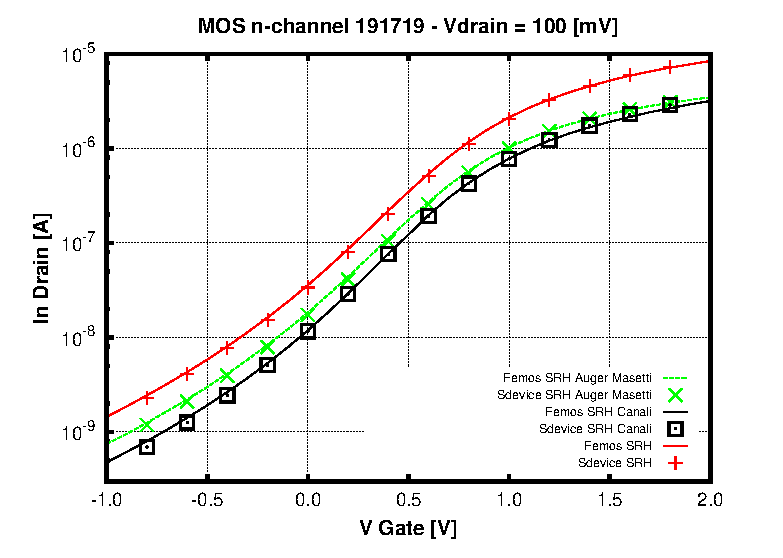
\includegraphics[scale=1]{CaratteristicheIV/MOS_Nchannel_191719_DIFFERENTMODELS}
\end{figure}

\clearpage 

\subsubsection{Bulk method}
Now the question is: it's possible extend the residue technique at the calculation of current inside the domain? The answer at this question is not trivial. A good start point is the work of J.R. Hughes and Larson in the article "The Continuous Galerikin Method Is Locally Conservative".The aim of their work is well exposed in the title and the conclusion is that this important property (locally conservation) is ensured less than the existence of an \textbf{auxiliary flux} denoted as $H(\omega)$ (with $\omega \subseteq\Omega$). 
To extract the statement of global and local conservation from the variational formulation, thay need to be able to set the weighting function to one. Obviously this is possible if $\Gamma_g=\varnothing$. In order to include every case an extended weak formulation is presented: consider $\eta$ the set of all verteces of the discrete domain and $\eta_g$ the subset of verteces on Dirichlet boundaries.
Now we are able to define the discrete space $\mathcal{V}^h:=span\{\psi_i\}_{i\in \eta - \eta_g} $ and  $V^h:=\mathcal{V}^h \oplus span\{\psi_i\}_{i\in \eta_g}$, where $\psi_i$ is the basis function assiociated with the node $i$.
The last space is the completion of the usual finite element space ($\mathcal{V}^h$). Note that the constant function having value 1 is contained in $V^h$. The modified form of Galerkin's method is given by:

Find $u^h\in \mathcal{S}^h$ and $H^h(\Omega)\in V^h - \mathcal{V}^h$ such that

\begin{equation}
\label{eq: extended weak formulation}
(W^h,H^h(\Omega))_{\Gamma_g}=B(W^h,u^h)-L(W^h) \psp{10} \forall W^h\in V^h
\end{equation}

Note that \referenzaeq{eq: extended weak formulation} splits into two subproblems:

\begin{equation}
\label{eq: usally problem}
0=B(w^h,u^h)-L(w^h) \psp{10} \forall w^h\in \mathcal{V}^h
\end{equation}
\begin{equation}
\label{eq: problem auxiliary flux}
(W^h,H^h(\Omega))_{\Gamma_g}=B(W^h,u^h)-L(W^h) \psp{10} \forall W^h\in V^h-\mathcal{V}^h
\end{equation}

Equation \referenzaeq{eq: problem auxiliary flux} is a problem which determines $H^h(\Omega)$. In it we assume $u^h$ is already determined by \referenzaeq{eq: usally problem}.
The coefficient matrix for \referenzaeq{eq: problem auxiliary flux} is the mass matrix associated with $\Gamma_g$

\begin{equation}
\sum_{j\in \eta_g} (\psi_i,\psi_j)H^h_j(\Omega) = B(\psi_i,u^h)-L(\psi_i) \psp{10} \forall i \in \eta_g
\end{equation}

\textcolor{red}{Il prodotto sul bordo genera la medesima matrice di massa?E cosa succede nei punti che non sono di Dirichlet?Non può essere formulato in questo modo il problema?}

In ogni caso noi abbiamo provato ad estendere il secondo problema ad ogni elemento interno che intersechi o meno i bordi di Dirichlet.
Questo a cosa corrsiponde?

Abbiamo interpretato la costruzione per elemento come se in ogni elemento il problema avesse delle condizioni di dirichlet che si affacciano con gli altri elementi adiacenti.
Se assumiamo che questa procedura sia corretta allora penso che i successivi ragionamenti stiano in piedi.

Sempre nell'articolo viene testata la formulazione estesa contro la funzione test costante e si ottiene la seguente equivalenza:

\begin{equation}
\int_{\Gamma_g}H^h(\Omega) \, d\Gamma = \int_{\Gamma^+_h}(a_nu^h-h^+) \, d\Gamma - \int_{\Gamma_h^-}h^- \, d\Gamma - \int_\Omega f \, d\Omega
\end{equation}

avendo assunto ogni nodo come Dirichlet allora valgono le seguenti affermazioni:
\begin{itemize}
\item $\Gamma_g = \partial \Omega$
\item $\Gamma_h = \varnothing$
\end{itemize}

quindi possiamo affermare che per ogni elemento vale:

\begin{equation}
\int_{\partial\Omega}H^h(\Omega) \, d\Gamma =  - \int_\Omega f \, d\Omega
\end{equation}

Ora vorrei ripartire dal problema di partenza:

\begin{equation}
\begin{array}{rcl}
-\nabla \cdot \vect{J} & = & f \\
\\
\int_\Omega -\nabla \cdot \vect{J} \Psi_k \, d\Omega & = & 
\int_\Omega f \Psi_k \, d\Omega  \psp{10}  \forall k = 1 ... N_{elements}\\
\\
\int_K -\nabla \cdot \vect{J} \, d\Omega & = & \int_K f \, d\Omega  \psp{10}  \forall k = 1 ... N_{elements}\\
\\
\int_{\partial K} -\vect{J} \cdot \vect{n} \, d\Omega & = & \int_K f \, d\Omega  \psp{10}  \forall k = 1 ... N_{elements}\\

\end{array}
\end{equation}

La domanda quindi \`e possiamo in qualche modo dire che:
\begin{equation}
H^h(K) = \vect{J}\cdot \vect{n} 
\end{equation}

Entrambe le quantit\`a sono definite sul bordo dell'elemento, inoltre la ricostruzione dalle componenti normali al vettore densit\`a di corrente non \`e impossibile.
Tuttavia occorre passare prima a definire la grandezza sulle facce del tetraedro:
\begin{itemize}
\item Calcolo delle quantit\`a nodali $H^h_j(\Omega)$
\item Redistribuzione dei valori sulle facce (metodo percentuale proporzionalmente alle aree) $\bar{H}^h_j(\Omega)$
\item Ortogonalizzazione dei contributi normali alle facce $\bar{H}^h_j(\Omega) \vect{n}_j$ tramite procedura alla Grand-Shmidt $H^*_j \vect{n}_j^*$
\item Calcolo del vettore densit\`a di corrente nell'elemento $\vect{J}=\sum_{i=1}^4 H^*_j\vect{n}_j^*$
\end{itemize}


%

%\section{The Residue Method}
%
%Riepilogo equazioni:
%
%\begin{array}{cc}
%\begin{cases} 
%-\nabla \cdot ( \vect{J}_n(n) ) = -qR & in \psp{3} \Omega \\ 
%-\nabla \cdot (\vect{J}_p (p)) = qR & in \psp{3} \Omega \\
%n = n_g & on \psp{3} \Gamma_g \\
%p = p_g & on \psp{3} \Gamma_g \\
%\nabla n \cdot \vect{n} = 0 & on \psp{3} \Gamma_n \\
%\nabla p \cdot \vect{n} = 0 & on \psp{3} \Gamma_n
%\end{cases}
%&
%\begin{equation*}
%\begin{array}{ccl}
%\vect{J}_n & = &- q\mu_n n \nabla \varphi + qD_n \nabla n \\
%\\
%\vect{J}_p & = & - q\mu_p p \nabla \varphi - qD_p \nabla p \\
%\\
%R(n,p) & = & (pn-n_i^2)(F_{SRH}(n,p)+F_{AU}(n,p)) \\
%&  &- (\alpha_n |\vect{v}_n|n + \alpha_p |\vect{v}_p|p)
%\end{array}
%\end{equation*}
%\end{array}
%
%\begin{equation}
%\begin{array}{l}
%\sigma_n(n,p) = qp(F_{SRH}(n,p)+F_{AU}(n,p)) \\
%\sigma_p(n,p) = qn(F_{SRH}(n,p)+F_{AU}(n,p)) \\
%f(n,p) = qn_i^2(F_{SRH}(n,p)+F_{AU}(n,p)) + q(\alpha_n |\vect{v}_n|n + \alpha_p |\vect{v}_p|p) 
%\end{array}
%\end{equation}
%
%
%\begin{equation}
%\begin{cases} 
%-\nabla \cdot ( \vect{J}_n(n) ) + \sigma_nn = f & in \psp{3} \Omega \\ 
%-\nabla \cdot (\vect{J}_p (p)) - \sigma_pp = -f & in \psp{3} \Omega \\
%n = n_g & on \psp{3} \Gamma_g \\
%p = p_g & on \psp{3} \Gamma_g \\
%\nabla n \cdot \vect{n} = 0 & on \psp{3} \Gamma_n \\
%\nabla p \cdot \vect{n} = 0 & on \psp{3} \Gamma_n
%\end{cases}
%\end{equation}
%
%Forme variazionali:
%\begin{equation}
%\begin{array}{c}
%B(v,n) = (\nabla v , \vect{J}_n(n))_{\Omega} + (\sigma_n n, v)_\Omega \\
%L(v) = (v,f)_\Omega
%\end{array}
%\end{equation}
%
%Spazi discreti:
%\begin{equation*}
%\mathcal{V}_h := span{\psi_i}_{i\in \eta_n} \psp{10} 
%V_h := span{\psi_i}_{i\in \eta_g} \psp{10}
%\mathbb{V}_h := V_h \oplus \mathcal{V}_h
%\end{equation*}
%
%Problema completo:
%\begin{equation}
%\label{eq: extended weak formulation}
%(W_h,H_h(\Omega))_{\Gamma_g}=B(W_h,n_h)-L(W_h) \psp{10} \forall W_h\in \mathbb{V}_h
%\end{equation}
%
%Problema diviso:
%\begin{equation}
%\label{eq: usally problem}
%0=B(w_h,n_h)-L(w_h) \psp{10} \forall w_h\in \mathcal{V}_h
%\end{equation}
%\begin{equation}
%\label{eq: problem auxiliary flux}
%(W_h,H_h(\Omega))_{\Gamma_g}=B(W_h,n_h)-L(W_h) \psp{10} \forall W_h\in V_h
%\end{equation}

\subsection{Idea}

Nel calcolo della corrente ai contatti si calcola sostanzialmente il residuo del problema DD globale, utilizzando per\`o la matrice di sistema non ancora modificata per le condizioni al bordo di Dirichlet. Infine dato un contatto (e quindi un insieme di vertici), si sommano le componenti del residuo relative ai vertici che risiedono su quel contatto. In questo modo otteniamo la corrente di elettroni $\mathcal{I}_n^k$ (k-esimo contatto). Possiamo affermare ovviamente che:
\begin{equation}
\mathcal{I}_n^k = \int_{\Gamma_k} \vect{J}_n \cdot \vect{n} \, d\Gamma_k
\end{equation}

Poniamo di aver risolto il problema e di conoscere le densit\`a su ogni vertice della triangolazione.\textbf{L'idea principale \`e di pensare ad ogni singolo elemento come un nuovo problema con condizioni di Dirichlet sui quattro vertici.} Applico nuovamente l'idea del calcolo della corrente ai contatti utilizzata per l'intero dominio di simulazione, ma questa volta ogni faccia del tetraedro costituisce un contatto. Quindi calcolo la matrice locale e la forzante locale del problema ed infine computo il residuo con la soluzione che gi\`a possiedo. Ora non mi resta che per ogni faccia (contatto) calcolare la corrente.

Assumendo $\vect{J}_n$ nel discreto essa \`e una quantit\`a definita sugli elementi, dunque sar\`a costante nel dominio che stiamo considerando in questo momento, possiamo affermare che data una faccia $k$ dell'elemento:

\begin{equation}
\mathcal{I}_n^k = \vect{J}_n \cdot \vect{n}_k |\Gamma_k|
\end{equation}

Cos\`i facendo \`e possibile recuperare quattro contributi alla corrente dell'elemento che tramite un'ortogonalizzazione alla Grand-Schmidt ci permettono di ricostruire il vettore densit\`a di corrente.

\begin{equation*}
\begin{array}{rcl}
\vect{J}_n  & = & \mathcal{I}_n^1 \vect{n}_1 
+ (\mathcal{I}_n^2 \vect{n}_2 - \mathcal{I}_n^2 (\vect{n}_2 \cdot \vect{n}_1) \vect{n}_1) \\
& & + (\mathcal{I}_n^3 \vect{n}_3 - \mathcal{I}_n^3 (\vect{n}_3 \cdot \vect{v}_2) \vect{v}_2 )
+ (\mathcal{I}_n^3 \vect{n}_3 - \mathcal{I}_n^3 (\vect{n}_3 \cdot \vect{n}_1) \vect{n}_1) \\
& & + (\mathcal{I}_n^4 \vect{n}_4 - \mathcal{I}_n^4 (\vect{n}_4 \cdot \vect{v}_3) \vect{v}_3 )
+ (\mathcal{I}_n^4 \vect{n}_4 - \mathcal{I}_n^4 (\vect{n}_4 \cdot \vect{v}_2) \vect{v}_2 )
+ (\mathcal{I}_n^4 \vect{n}_4 - \mathcal{I}_n^4 (\vect{n}_4 \cdot \vect{n}_1) \vect{n}_1)
\end{array}
\end{equation*}

Mi sembra una possibile estensione del metodo dei residui all'interno del dispositivo anche se probabilmente potrei avere commesso degli errori nello sviluppo dell'idea. Tuttavia anche nel caso di una corretta base teorica, per come ho presentato il metodo mi sembra che si rischi di incorrere in problemi numerici date le numerosi differenze che occorrerebbe fare.

Probabilmente aiutandoci con gli articoli di Hughes possiamo tirar fuori un'idea simile, sfruttando in qualche modo i flussi ausiliari che sono senza dubbio legati ai residui dei problemi locali.

%
%\clearpage
%
%\section{First results}
%
%
%\clearpage
%
%
%\chapter{Dual mixed method (or thermo electric system?)}

%\addcontentsline{toc}{chapter}{Bibliografia}
\bibliographystyle{alpha}
\bibliography{libri}

\end{document}